\section{Описание}

В качестве задачи выбрана задача по бинарной классификации астрономических объектов согласно датасету \href{https://www.kaggle.com/datasets/colearninglounge/predicting-pulsar-starintermediate}{Predicting Pulsar Star}.

Датасет направлен на определение пульсаров, и описывает каждый объект при помощи следующих признаков:

\begin{enumerate}
	\item Mean of the integrated profile --- среднее значение усредненного профиля импульса
	\item Standard deviation of the integrated profile --- отклонение усредненного профиля импульса
	\item Excess kurtosis of the integrated profile --- эксцесс усредненного профиля импульса
	\item Skewness of the integrated profile --- асимметрия усредненного профиля импульса
	\item Mean of the DM-SNR curve --- среднее значение кривой DM-SNR
	\item Standard deviation of the DM-SNR curve --- отклонение кривой DM-SNR
	\item Excess kurtosis of the DM-SNR curve --- эксцесс кривой DM-SNR
	\item Skewness of the DM-SNR curve --- асимметрия кривой DM-SNR
	\item Class --- целевое значение
\end{enumerate}

\section{Ход работы}

Датасет содержит в себе данные о восьми параметрах объекта и его класс.

\begin{lstlisting}[frame=none, numbers=none]
RangeIndex: 12528 entries, 0 to 12527
Data columns (total 9 columns):
 #   Column           Non-Null Count  Dtype  
---  ------           --------------  -----  
 0   Mean IP          12528 non-null  float64
 1   Std IP           12528 non-null  float64
 2   Kurtosis IP      10793 non-null  float64
 3   Skewness IP      12528 non-null  float64
 4   Mean DM-SNR      12528 non-null  float64
 5   Std DM-SNR       11350 non-null  float64
 6   Kurtosis DM-SNR  12528 non-null  float64
 7   Skewness DM-SNR  11903 non-null  float64
 8   class            12528 non-null  int32
\end{lstlisting}

Все признаки являются количественными, дополнительного кодирования не требуется. Видно, что данные неполные, рассмотрим это подробнее.

\begin{lstlisting}[frame=none, numbers=none]
Mean IP               0
Std IP                0
Kurtosis IP        1735
Skewness IP           0
Mean DM-SNR           0
Std DM-SNR         1178
Kurtosis DM-SNR       0
Skewness DM-SNR     625
class                 0
\end{lstlisting}

В качестве борьбы с пропусками удалим все строки, в которых они обнаружены. В результате данных станет немного меньше.

Визуализируем признаки при помощи гистограмм:

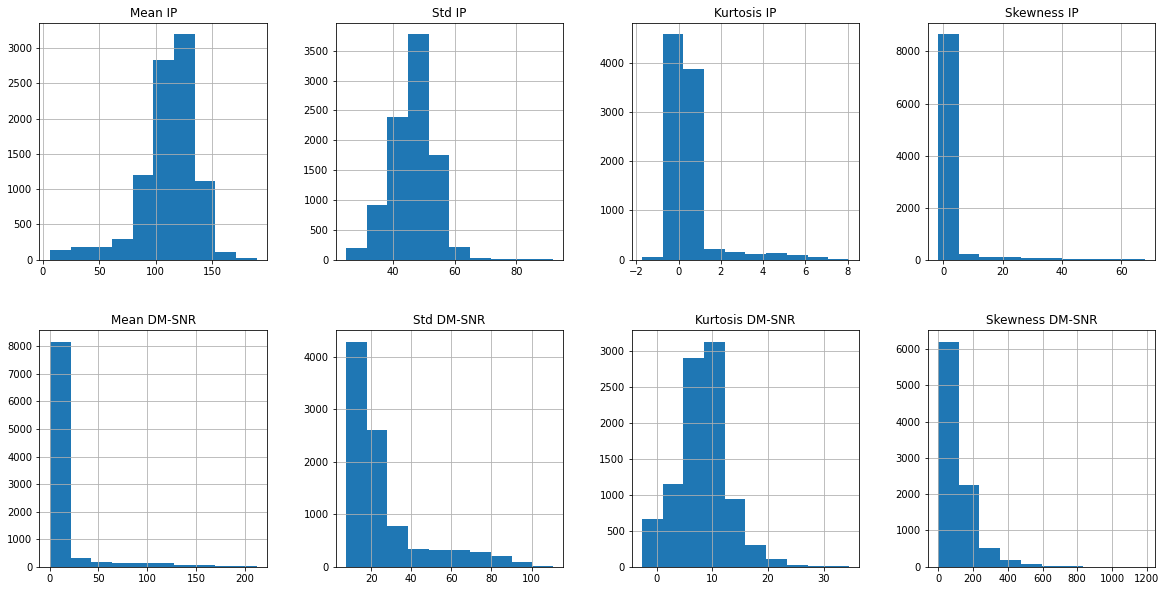
\includegraphics[width=\textwidth]{hist}

В распределениях признаков не наблюдается аномальных отклонений.
\pagebreak

Подсчитаем коэффициенты корреляции между признаками:

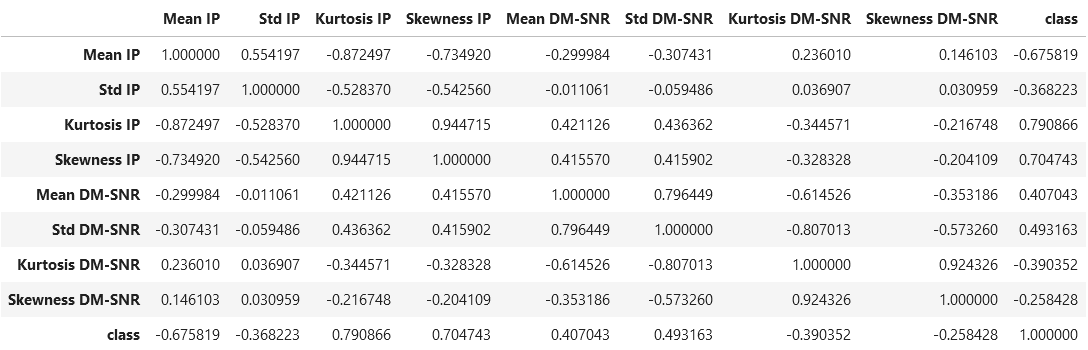
\includegraphics[width=\textwidth]{corr_table}

Также в виде тепловой карты:

\begin{figure}[h]
\centering
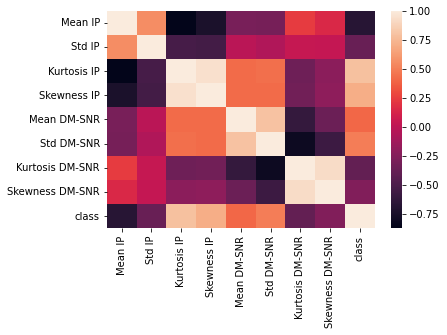
\includegraphics[scale=0.5]{corr_heatmap}
\end{figure}

Видно, что некоторые признаки коррелируют друг с другом. Вероятно это связано с тем, что они представляют из себя статистические характеристики других данных. Отдельно отметим коэффиценты корреляции между признаками и целевым значением.

\begin{lstlisting}[frame=none, numbers=none]
Mean IP           -0.675819
Kurtosis DM-SNR   -0.390352
Std IP            -0.368223
Skewness DM-SNR   -0.258428
Mean DM-SNR        0.407043
Std DM-SNR         0.493163
Skewness IP        0.704743
Kurtosis IP        0.790866
\end{lstlisting}

Имеются три признака с высокой корреляцией: Mean IP, Skewness IP, Kurtosis IP --- их можно считать наиболее выжными. Это говорит о возможности использования линейных моделей.
\pagebreak

Также построим попарные графики зависимостей для всех признаков:

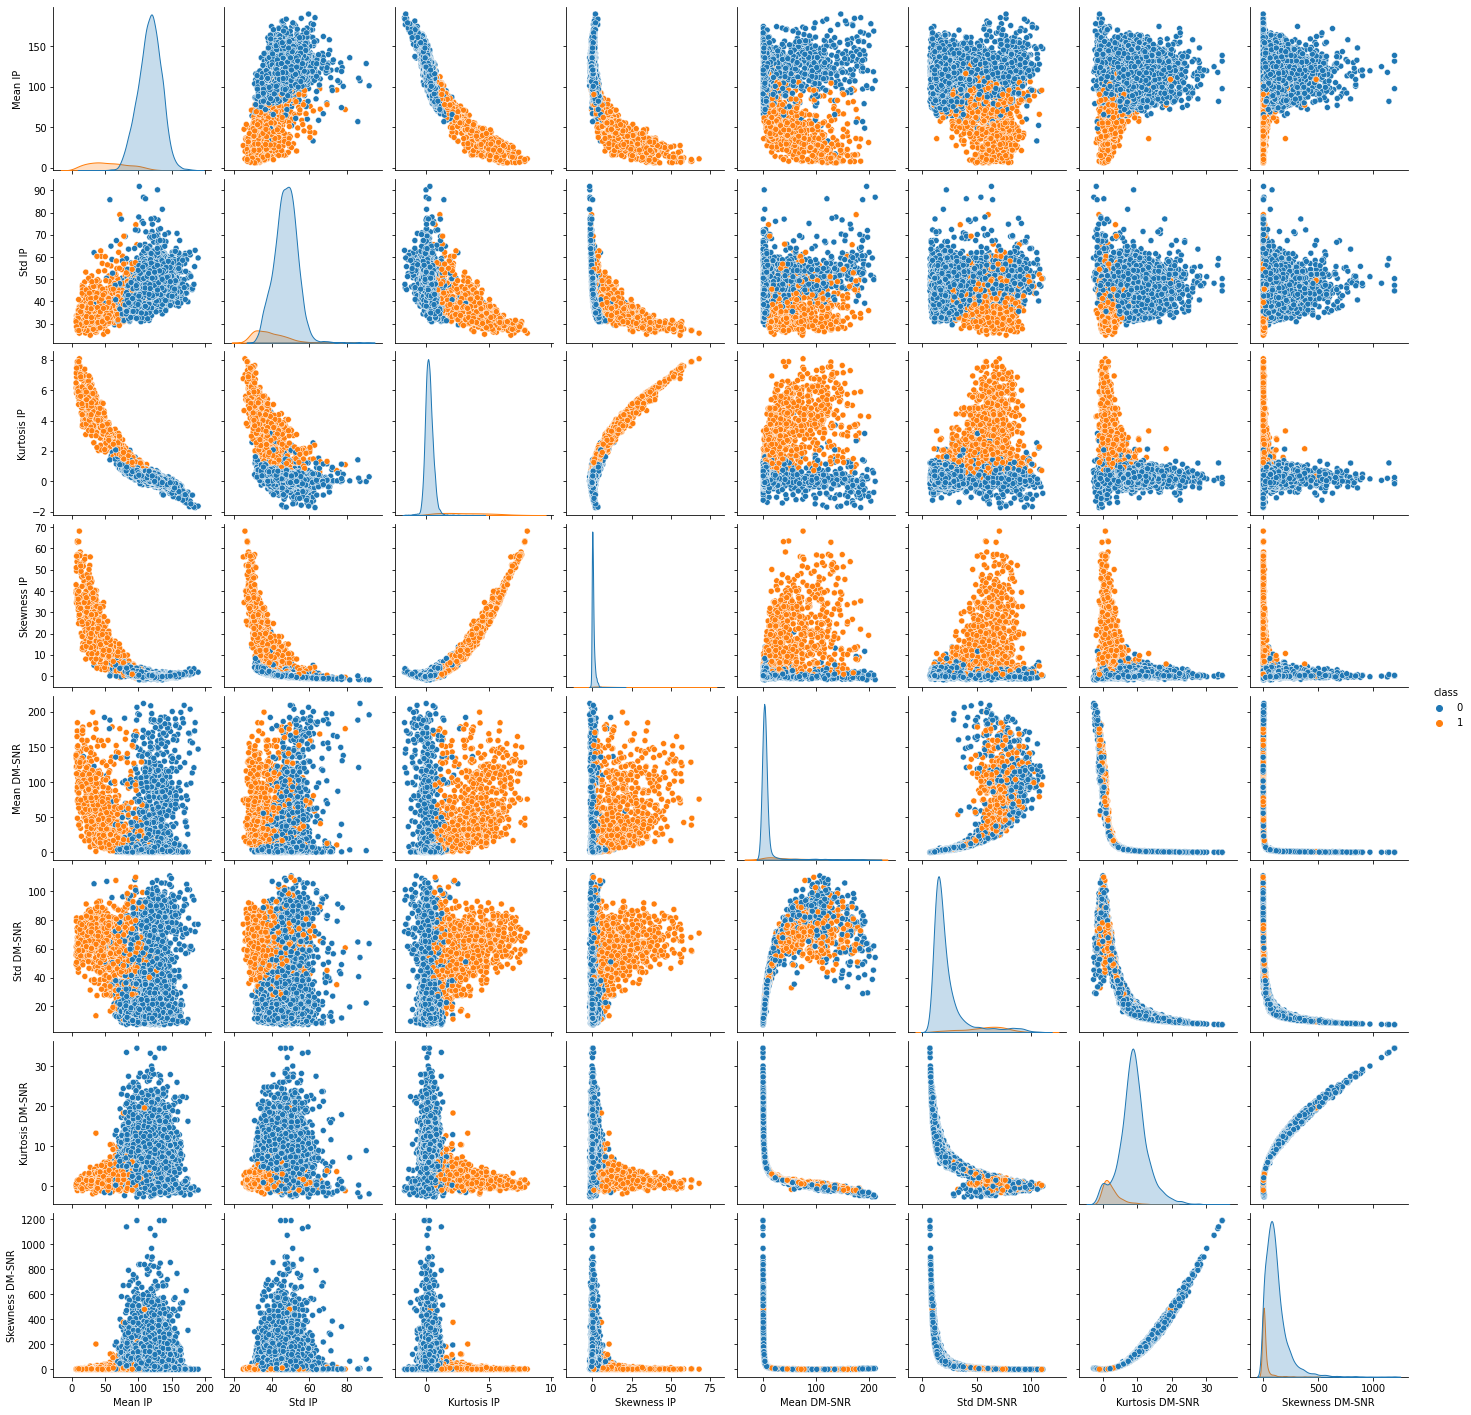
\includegraphics[width=\textwidth]{pairplot}

Такие графики подтверждают предыдущие выводы. На них видно и сильно коррелирующие признаки, и то, что на графиках признаков с высокой корреляцией с целевым значением, объекты разных классов можно достаточно хорошо разделить прямой. Отсюда также можно сделать вывод об отсутствии необходимости составления новых признаков.
\pagebreak

Важным параметром датасета является соотношение между классами.

\begin{figure}[h]
\centering
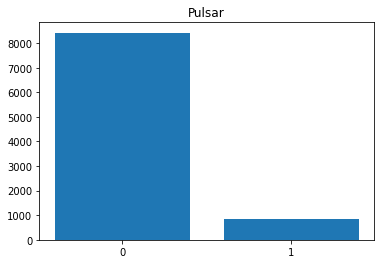
\includegraphics[scale=0.5]{barplot_before}
\end{figure}

Данные сильно несбалансированны, что плохо повлияет на обучение. Применим оверсэмплинг.

\begin{lstlisting}[language=python, keepspaces=true]
sample = data[data['class'] == 1]
while data[data['class'] == 1].shape[0] + sample.shape[0] < 
      data[data['class'] == 0].shape[0]:
    data = pd.concat([data, sample])

data = pd.concat([data, sample.iloc[:data[data['class'] == 0].shape[0] - 
                                     data[data['class'] == 1].shape[0]]])
\end{lstlisting}

После оверсэмплинга:

\begin{figure}[h]
\centering
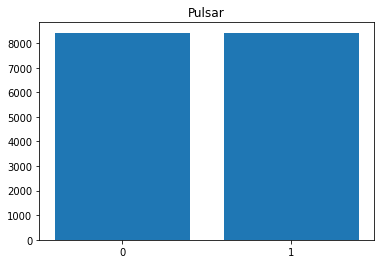
\includegraphics[scale=0.5]{barplot_after}
\end{figure}

\pagebreak

